\documentclass{beamer}

\usepackage{beamerthemesplit}
\usetheme{Singapore} %Copenhagen}
%\usecolortheme{whale}

%\usepackage[T2A]{fontenc}
%\usepackage[utf8]{inputenc}
%\usepackage[russian]{babel}

\usepackage[main=russian,english]{babel}   %% загружает пакет многоязыковой вёрстки
\usepackage{fontspec}      %% подготавливает загрузку шрифтов Open Type, True Type и др.
\defaultfontfeatures{Ligatures={TeX},Renderer=Basic}  %% свойства шрифтов по умолчанию
\setmainfont{Times New Roman} %% задаёт основной шрифт документа
%\usefonttheme{professionalfonts}% SOLUTION
\usefonttheme{serif}

\usepackage{hyperref}
\usepackage{textcomp}
\usepackage{amssymb,amsmath}
%\usepackage{animate}
%\usepackage{longtable}
\usepackage{xcolor}

%\usepackage{pgffor}
\usepackage{enumitem}


\newcounter{N}

%% Форматирование окружения itemize
%\usepackage{ragged2e}
%\let\olditem\item
%\renewcommand\item{\olditem\justifying}


\newcommand{\argxi}{(\xi^1,\xi^2,\xi^3)}
\newcommand{\argx}{(x^1,x^2,x^3)}

\newcommand{\argxbarn}{(\bar{x}^1,\bar{x}^2,\ldots, \bar{x}^n)}
\newcommand{\argxn}{(x^1, x^2,\ldots, x^n)}

\newcommand{\argtxi}{(t, \xi^1,\xi^2,\xi^3)}
\newcommand{\argtoxi}{(t_0, \xi^1,\xi^2,\xi^3)}

\newcommand{\argtx}{(t, x^1,x^2,x^3)}
\newcommand{\argtox}{(t_0, x^1,x^2,x^3)}

\newcommand{\pd}[2]{\frac{\partial #1}{\partial #2}}
\newcommand{\pdk}[2]{\frac{\partial^2 #1}{\partial {#2}^2}}

\title[]{Cилы, действующие на сплошную среду, тензор напряжений}

\author[]{ {\em Верещагин Антон Сергеевич}
\\
канд. физ.-мат. наук, старший преподаватель\\
\bigskip
Кафедра аэрофизики и газовой динамики ФФ НГУ}

\usebackgroundtemplate{\includegraphics[width=\paperwidth]{../img/background.png}}

\begin{document}
	
\frame{\titlepage}


\frame{
	\frametitle{Аннотация}
	\parbox{\textwidth}{
	}
}

\frame{
	\frametitle{ Объемные и массовые силы }
	
	\begin{exampleblock}{Определение }
		\parbox{\textwidth}{
			Силы, действующие на каждый элемент объема $d\omega$ независимо от того, существуют ли рядом с объемом $d\omega$ другие частицы или нет, называются  \alert{объемными}. 	Если такие силы отнесены к единице массы, то они называются \alert{массовыми}.
		}
	\end{exampleblock}\pause

	\begin{exampleblock}{Пример}
		\parbox{\textwidth}{
		Объемная сила, действующая на частицу среды в поле силы тяжести, определяется соотношением
		\[
		d\vec{F} = \rho \vec{g} d\omega,
		\]
		где $\rho$ -- плотность жидкой частицы, $\vec{g}$ -- вектор ускорения свободного падения.
		}
	\end{exampleblock}
}

\frame{
	\frametitle{ Поверхностные силы }
	
	\begin{columns}
		\begin{column}{0.35\textwidth}
			\parbox{\textwidth}{
				\centering
				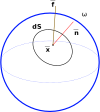
\includegraphics[width=\textwidth]{../img/sigma_def.pdf}
				
				\medskip	
				\scriptsize
				\parbox{\textwidth}{
				Выделенный объем сплошной среды $\omega$, с фиксированной точкой $\vec{x}$ внутри него и элементарной площадкой $dS$ с единичной нормалью $\vec{n}$		

				}

			}
		\end{column}
		\begin{column}{0.65\textwidth}
			\begin{exampleblock}{Определение }
				\parbox{\textwidth}{
					\alert{Напряжением поверхностной силы} $\vec{f}$ называется величина силы, отнесенная к элементарной площадке $dS$ с единичной нормалью $\vec{n}$, возникающая в результате взаимодействия частей среды с разных сторон от элементарной площадки в малой окрестности точки $\vec{x}$. 
				}
			\end{exampleblock}
		

		\end{column}
	\end{columns}
}

\frame{
	\frametitle{ Поверхностные силы  }
		\begin{columns}
		\begin{column}{0.35\textwidth}
			\parbox{\textwidth}{
				\centering
				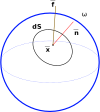
\includegraphics[width=\textwidth]{../img/sigma_def.pdf}
				
				\medskip	
				\scriptsize
				\parbox{\textwidth}{
					Выделенный объем сплошной среды $\omega$, с фиксированной точкой $\vec{x}$ внутри него и элементарной площадкой $dS$ с единичной нормалью $\vec{n}$					
				}
				
			}
		\end{column}
		\begin{column}{0.65\textwidth}
			
			\begin{exampleblock}{Замечания}
				\parbox{\textwidth}{
					\begin{itemize}[partopsep=1pt,label=\textbullet]
						\item Поверхностная сила существует в каждой точке среды (как на поверхности, так и на границе).
						\item Поверхностная сила является функцией точки среды $\vec{x}$ и ориентации площадки  $\vec{n}$:
						\[
						\vec{f} = \vec{f}(\vec{x},\vec{n}).
						\]
						\item Считаем, что $\vec{n}$ -- вектор внешней единичной нормали.
					\end{itemize}
				}
			\end{exampleblock}
		\end{column}
	\end{columns}
}


\frame{
	\frametitle{ Поверхностные силы  }
	\begin{columns}
		\begin{column}{0.35\textwidth}
			\parbox{\textwidth}{
				\centering
				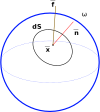
\includegraphics[width=\textwidth]{../img/sigma_def.pdf}
				
				\medskip	
				\scriptsize
				\parbox{\textwidth}{
					Выделенный объем сплошной среды $\omega$, с фиксированной точкой $\vec{x}$ внутри него и элементарной площадкой $dS$ с единичной нормалью $\vec{n}$					
				}
				
			}
		\end{column}
		\begin{column}{0.65\textwidth}
			
			\begin{exampleblock}{Замечания}
				\parbox{\textwidth}{
					\begin{itemize}[partopsep=1pt,label=\textbullet]
						\item Для определения суммарной силы, действующей на объем $\omega$, ограниченного поверхностью $S$, необходимо проинтегрировать $\vec{f}(\vec{x},\vec{n}(\vec{x}))$ по этой поверхности:
						\[
						\vec{F} = \int\limits_{S}\vec{f}(\vec{x},\vec{n}(\vec{x}))dS.
						\]
					\end{itemize}
				}
			\end{exampleblock}
		\end{column}
	\end{columns}
}

\frame{
	\frametitle{ Принцип равенства действий и противодействий  }

	\centering
	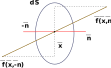
\includegraphics[width=0.5\textwidth]{../img/surface_action.pdf}\\
	{
		\scriptsize
		Иллюстрация равенства напряжения на противоположных направлениях		
	}	

	\bigskip
	\parbox{\textwidth}{
	Если рассмотреть напряжения, возникающие в точке $\vec{x}$ на площадке с единичной нормалью $\vec{n}$ и ей противоположной, то в следствие принципа равенства действия и противодействия
	\[
	\vec{f}(\vec{x},\vec{n}) = -\vec{f}(\vec{x},-\vec{n}).
	\]		
	}
}
\frame{
	\frametitle{Разложение напряжения}
	
	\begin{columns}
		\begin{column}{0.5\textwidth}
			\centering
			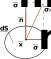
\includegraphics[width=0.7\textwidth]{../img/sigma_decomposition.pdf}
			
			\scriptsize
			Разложение напряжения на нормальную и тангенциальную составляющие
		\end{column}
		\begin{column}{0.5\textwidth}
			\parbox{\textwidth}{
			Напряжение в точке $\vec{x}$, возникающее на площадке $dS$ с единичной нормалью $\vec{n}$, можно представить в виде суммы нормальной $\vec{f}_n$ и тангенциальной составляющих $\vec{f}_\tau$:
			\[
			\vec{f} = \vec{f}_n+\vec{f}_\tau.
			\]
			
			В этом случае $\vec{f}_n$ называется \alert{нормальным растяжением} или \alert{нормальным давлением}. $\vec{f}_\tau$ называют \alert{косым напряжением} или \alert{силой трения}.
			}
		\end{column}
	\end{columns}
	
}

\end{document}
